%%%%%%%%%%%%%%%%%%%%%%%%%%%%%%%%%%%%%%%%%%%%%%%%%%%%%%%%%%%%%%%%%%%%%%%%%%%%%%%%
%2345678901234567890123456789012345678901234567890123456789012345678901234567890
%        1         2         3         4         5         6         7         8

\documentclass[letterpaper, 10 pt, conference]{ieeeconf}  % Comment this line out if you need a4paper
\usepackage{graphicx}
\usepackage{amsmath}
\usepackage{url}
%\documentclass[a4paper, 10pt, conference]{ieeeconf}      % Use this line for a4 paper

\IEEEoverridecommandlockouts                              % This command is only needed if 
                                                          % you want to use the \thanks command

\overrideIEEEmargins                                      % Needed to meet printer requirements.
\usepackage{listings} 
% See the \addtolength command later in the file to balance the column lengths
% on the last page of the document

% The following packages can be found on http:\\www.ctan.org
%\usepackage{graphics} % for pdf, bitmapped graphics files
%\usepackage{epsfig} % for postscript graphics files
%\usepackage{mathptmx} % assumes new font selection scheme installed
%\usepackage{times} % assumes new font selection scheme installed
%\usepackage{amsmath} % assumes amsmath package installed
%\usepackage{amssymb}  % assumes amsmath package installed

\title{\LARGE \bf
As Autonomous As Possible: POMDPs for Risk-Aware Reinforcement Learning.
}


\author{William Curran$^{1}$, Cameron Bowie$^{1}$ and William D. Smart $^{1}$% <-this % stops a space
\thanks{$^{1}$William Curran, Cameron Bowie and William D. Smart are with the Robotics Program in the School of Mechanical, Industrial and Manufacturing Engineering, Oregon State University, Corvallis, OR 97330, USA.
{\tt\small curranw@onid.orst.edu, bowiec@onid.orst.edu, bill.smart@oregonstate.edu}}%
}

\begin{document}



\maketitle
\thispagestyle{empty}
\pagestyle{empty}


%%%%%%%%%%%%%%%%%%%%%%%%%%%%%%%%%%%%%%%%%%%%%%%%%%%%%%%%%%%%%%%%%%%%%%%%%%%%%%%%
\begin{abstract}

%Risk-sensitive reinforcement learning is a well established yet often over zealous approach to learning in new environments. Using these traditional approaches, dangerous or undesirable states are entirely avoided. This assumes that an efficient autonomous approach exists for the task being performed. However, developing full autonomy for all tasks in all environments is simply not possible with today's technology, even with risk-aversion. An autonomous approach already exists for many tasks, but can not be guaranteed to always succeed. These rare, yet important failures are important to represent when choosing between different approaches. 

Autonomous approaches are effective, but do not work in every environment. Autonomy suffers in situations when computer vision fails, or when the learned task is too dissimilar to the current task. Knowing the risk of using an autonomous or alternative approach is important when deciding how to perform a task. In this work, we introduce $A^3P$, a risk-aware task-level reinforcement learning algorithm. $A^3P$ represents a task-level state machine as a POMDP. In this POMDP tasks are states and approaches are actions. Failures are represented in the learned solution as additional state-action pairs, allowing the user to make more informed decisions when choosing between different approaches. We demonstrate $A^3P$ in a corridor domain problem and test the true learning distributions to the learned. We find that $A^3P$ learns an accurate and risk-aware policy for the corridor problem domain.
\end{abstract}

 
%%%%%%%%%%%%%%%%%%%%%%%%%%%%%%%%%%%%%%%%%%%%%%%%%%%%%%%%%%%%%%%%%%%%%%%%%%%%%%%%
\section{INTRODUCTION}

As robots become more commonplace in our homes and workplaces, their ability to adapt to new environments and perform novel tasks becomes paramount. Autonomy allows the robot to work for an extended period of time without human intervention. The autonomous execution of many tasks are performed more efficiently when compared to manual teleoperation. 

Autonomy works well in controlled environments with robot-friendly affordances. However, engineers design most devices with a human user in mind. Turning small black dials on a black stereo system is a difficult task for a robot to do autonomously. Additionally, without the user in control of the robot, the autonomous system must perform image processing, path planning, object manipulation routines, and more in order to accomplish the task. This typically requires a lot of computation, reduces battery life, and diminishes the robot's ability to parallelize physical tasks. Autonomy can also be error-prone in new environments. Developing full autonomy for all tasks in all environments is simply not possible with today's technology. Despite recent advances in the field of autonomous robotics \cite{darpa, 6343870, 5980259}, we are still many years away from a fully autonomous adaptive robot.

By applying a shared autonomy approach, we can separate low-level reactivity from higher-level reasoning, and give the latter to a human operator in cases where an autonomous system might perform poorly. This gives the user more direct control over the robot, relieving many of the issues of pure autonomy \cite{Goodrich:2007:HIS:1348099.1348100}. It also allows the robot to perform effectively in new environments without extensive reprogramming. Robots tend to be error-prone, but shared autonomy alleviates this through collaboration \cite{5980259}. 

%Using shared autonomy and teleoperation reduces the computational burden on the robot by having the human operator perform complex perception and decision-making tasks, and giving them manual control over the robot. This is a good approach when the robot is under a high CPU load or the user needs to perform a complex task in a specific way. This approach also allows a robot to effectively perform in new environments, but requires the user's full attention and responsive control.

In this paper, we present As Autonomous as Possible ($A^3P$), an algorithm that autonomously selects from a set of approaches to use when performing parts of a given task. By combining reinforcement learning with a task-level state machine architecture, we are able to learn risks associated with each approach. This allows us to make an informed decision and better balance execution time and risk. We represent tasks as state machines, and make decisions about whether to use autonomy, shared autonomy, or teleoperation for each of the states, depending on which is most effective for the given sub-task.  As new autonomous capabilities emerge, we can easily add them to this model, and have $A^3P$ automatically incorporate them.

%Each state in the state machine represents one or more teleoperation, shared autonomy or full autonomy approaches. As we start developing multiple methods of accomplishing the same task, being able to autonomously decide which approach to use becomes important.

Being risk-averse is also an important aspect in robotics. Many autonomous approaches fail some small percentage of the time, or take much longer to perform the task due to some changed environmental condition (i.e. lighting). Currently, reinforcement learning uses rewards to develop a long-term average representing the value of an action in specific state. By using a long-term average, reward outliers are lost. In this work, we want to find the optimal action in relation to the risk associated with that action. Therefore, we develop a reinforcement learning algorithm that represents these outliers and underlying transition functions, essentially allowing the user to choose the robot's level of risk. 

%We use $A^3P$ in four key ways: 
%\begin{itemize}
%\item Autonomously detect which approaches do not work in a specific environment.
%\item Autonomously detect which approach is inefficient at the task.
%\item Discern which approach works best given the current environment.
%\item Develop a cost-benefit risk analysis.
%\end{itemize}

%We experimentally validate the effectiveness of our approach with a standard navigation problem.

To experimentally validate $A^3P$ we use a standard navigation problem. In this problem a simulated robot must navigate through a corridor and perform a task. We add an optional shortcut through a narrow doorway with an associated error rate (Figure \ref{Corridor}). The narrow doorway represents the cost-benefit risk analysis, as the robot may have difficulty navigating with precision, or something may be blocking the doorway. We test the efficacy of our approach by empirically analyzing the convergence of $A^3P$, directly comparing the true learning solution to our learned solution, and comparing a traditionally-learned policy to our risk-averse policy.

We organize the remainder of this paper as follows. Section II describes the related work in robot autonomy, reinforcement learning and SMACH. Section III contains the key contribution of this work, $A^3P$, and describes the basic algorithm. In Section IV we describe the experimental validation approach and empirical results, followed by the conclusion in Section V.


\section{BACKGROUND}

To motivate our approach, we outline previous work performed in the field of robot autonomy, describe the reinforcement learning technique used in this work, and give an overview the current SMACH infrastructure.

\subsection{Robot Autonomy and Teleoperation}

In robotic competitions typically full autonomy is the ultimate goal for robotic systems \cite{darpa}. With full autonomy, the user only intervenes with the robot on the tasking level. The user allocates tasks to a robot and trusts it to complete those tasks without any additional intervention. This dramatically increases the efficiency many tasks, which is valuable in many disciplines. 

However, autonomy suffers in situations when computer vision fails, or when the learned task is too dissimilar to the current task. When performing manipulation tasks, the approach must use object detection or segmentation. These computer vision techniques assist the robot to find the location, shape and size information of devices. By using these device attributes and shape primitives, the robot can accurately manipulate the object. Even though there is a large research focus toward these computer vision techniques, the methods do not robustly detect objects in difficult scenes \cite{5980259}.  

When autonomy fails, the user can waste more time than if they simply teleoperated the robot, or completed the task themselves, and damage can occur to the robot or the surroundings. This adds a large cost to autonomous failures. Despite this cost, the benefits of using autonomy greatly outweigh the benefits of using other approaches \cite{6343870}, and roboticists should use them if available.

By using shared autonomy, designers can separate the low-level reactivity from the higher level reasoning, and give the higher level reasoning task to the user. Human users are skilled at classifying objects in the world and performing high-level task-based reasoning and can use these abilities to advise the robot \cite{goodfellow_help_2010}. By telling the robot the shape, location and size of the object to manipulate, the robot can then easily perform the task.

Shared autonomy is an effective compromise when autonomy is not practical, but it still requires the attention of the user. Shared autonomy requires an implementation for each type of question or prompt and requires a high-level decision making ability to determine which question to ask. Furthermore, the ability to understand and predict robot behavior is important, but may not be intuitive in autonomous approaches.

%Both autonomy and shared autonomy involves a high CPU load cost. Performing image processing, path planning, mapping, localization, high degree of freedom arm trajectory planning, and low and high-level decision making simultaneously inflicts a very large CPU load on the robot, making parallel computations become slow. Teleoperation removes much of this computation overload by giving the user complete control.  

During teleoperation, a user controls a robot via an interface to perform a complex task \cite{Dragan_2013_7390}. Teleoperation's predictability and robustness to environmental changes makes it the traditional approach for robotic movement. There exists a variety of interfaces for many robot types, such as ground vehicles \cite{6256067}, aerial vehicles \cite{helicopter}, wheelchair arms \cite{1639157}, and many more.

However, teleoperation is often tedious and difficult \cite{Dragan_2013_7390}. The user must work through an interface that is different from actual human motion to accomplish a complex task. In addition, the robots sensors provide a limited field of view. Due to this inability to understand the robots position or perspective within the environment, it is difficult for users to navigate effectively \cite{Bruemmer:2005:SUC:2229264.2230046}.

\subsection{Reinforcement Learning}
The Markov Decision Process (MDP) models a fully-observable sequential decision processes. A MDP is a 4-tuple $(S,A,P,R)$, where $S$ is a finite set of states, $A$ is a finite set of actions, $P$ is the probability that a certain action $a$ leads from state $s$ to state $s'$ and $R$ is the reward obtained from taking action $a$ in state $s$ resulting in state $s'$. 

A POMDP is a generalized partially-observable extension of the MDP. A POMDP is a 6-tuple $(S,A,O, T, \gamma, R)$, where $S$, $A$, and $R$ are the same as a MDP, $O$ is a set of observations, $T$ is a set of conditional transition probabilities and $\gamma$ is a set of conditional observation probabilities. In a POMDP, the agent cannot directly observe the underlying state, and must probabilistically determine its state. In this work we use a POMDP framework with reinforcement learning.

Reinforcement learning is a tool within the field of multiagent or single-agent learning where agents take an action, observe the environment, and receive a reward based on the new environment \cite{Sutton98reinforcementlearning}. Reinforcement learning finds an optimal policy, $\pi(s,a) = P(a|s)$, that maximizes a reward function, $R$.

To develop this optimal policy, reinforcement learning uses the current state of the agent, $s$, the action taken, $a$, the resultant state, $s'$, and a reward corresponding to the system-level success or failure of the state and action, $R$.

%There are three main aspects when defining a stateful reinforcement learner: the policy, the reward function, and the state transitions. 

The reinforcement learner's policy represents the actions an agent should take in each state. Learning algorithms based on value functions estimate a value function $Q^\pi(s,a)$ that computes the long-term reward of state $s$ to derive a policy $\pi(s)$ \cite{Kalyanakrishnan:2009:EAV:1558109.1558115}. In this work we use Q-Learning \cite{Sutton98reinforcementlearning}:

\begin{align*}
Q_{t+1}(s_t,a_t) \leftarrow & Q_t(s_t,a_t) + \alpha [R_{t+1}(s_t,a_t) \\
 & + \gamma \max_a Q_t(s_{t+1},a) - Q_t(s_t,a_t)]
\end{align*}
with values represented in a discrete tabular structure known as the Q-Table. We also enforce $\epsilon$-greedy action selection, where the best action is chosen with probability $1 - \epsilon$ and a random action with probability $\epsilon$.

The reward function encompasses the high-level goal of the system. When an agent takes an action that is good for the system, the reward function returns to the agent a positive reward proportional to how much it helped the system-level reward. Reinforcement learners also receive a correspondingly smaller reward when their actions are detrimental to the system. In this way agents can iteratively update to converge to the optimal policy according to their reward design.

Risk-sensitive reinforcement learning typically represents risk states as error states \cite{Geibel:2005:RRL:1622519.1622522}, are only concerned with the variance \cite{Borkar:2002:QRC:767822.769466, Liu:2003:RAA:860575.860632} or worst-case reward outliers \cite{Coraluppi1999301}. In this work we deal with already learned approaches. These approaches typically have an error rate, causing large reward outliers. We represent these reward outliers as risk in the learning problem, and let the user decide their own level of risk-averseness.

\subsection{SMACH}
SMACH \cite{smach} is a task-level architecture for creating complex robot behavior. It uses a hierarchical state machine infrastructure to represent the states and state transitions associated with complex tasks. A programmer can use this infrastructure to easily debug each independent state, as well as plug-and-play states for different applications.  

SMACH is a Robot Operating System (ROS) \cite{288} package that has been used in a variety of complex tasks, mainly on the PR2 platform. Using SMACH, researchers have been able to quickly prototype tasks such as retrieving drinks from a refrigerator, autonomously plugging in (Figure 1), and playing pool. 

We extend the SMACH framework to allow programmers to add multiple state transition options with the same state outcome. The $A^3P$ infrastructure then uses reinforcement learning to decide which state transition to take.

\begin{figure}
\centering
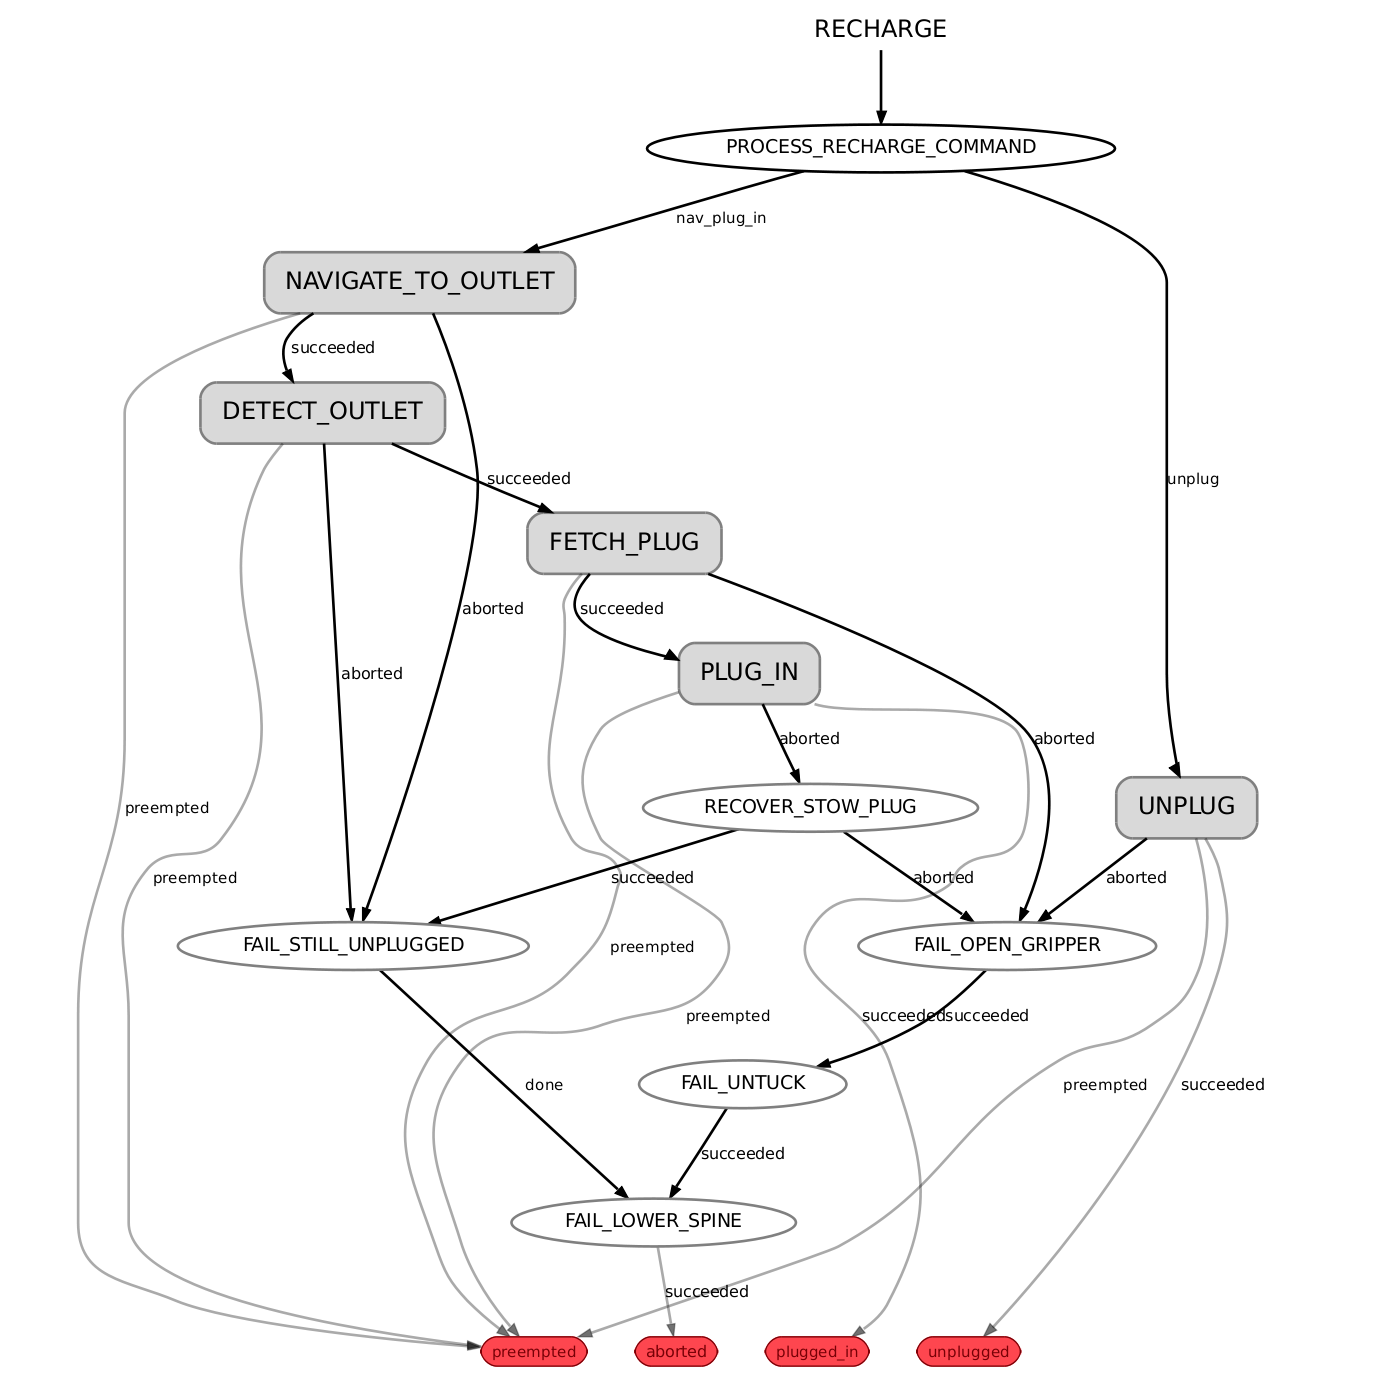
\includegraphics[width=.75\columnwidth]{smach.png}
\caption{Example SMACH state machine used to allow the PR2 robot to charge itself.}
\label{SMACH}
\end{figure}
   
\section{As Autonomous As Possible}
In this section we describe the As Autonomous As Possible ($A^3P$) algorithm. We first describe a general overview of $A^3P$ and implementation details. We then discuss the learning details built into the $A^3P$ algorithm. 

\subsection{$A^3P$ Overview}
In this work we introduce a risk-aware task-level reinforcement learning algorithm that can adapt an end-user's risk tolerance. $A^3P$ learns a task-level policy where states are sub-tasks and actions are approaches in accomplishing that sub-task. We cannot apply reinforcement learning to this type of problem, as many state-action pairs have extreme reward outliers we want to represent. For example, when a robot executes a task, teleoperation errors, object opacity, lighting conditions and more affect the efficiency of execution. These cause an extreme outlier in the reward function. In direct reinforcement learning, non-outlier rewards eventually outweigh this outlier, and it becomes lost in the average. We want the converged Q-Table to also represent these extreme outliers, rather than only the long-term averages.  

First, we assume that all reward sampling is from a Gaussian distribution. We can make this assumption because rewards are based on time. Every task a human or computer executes can be accomplished a stochastic amount of time, and we assume these distributions can be represented by a Gaussian. 

\begin{figure*}
\vspace*{0.1in}
\centering
\includegraphics[width=1.8\columnwidth]{code_snippet}
%\lstset{language=Python}          % Set your language (you can change the language for each code-block optionally)
%
%\begin{lstlisting}[frame=single, showstringspaces=false,linewidth=18cm]  % Start your code-block
%
%def main():
%  sm_top = smach.StateMachine(outcomes=`done')
%  with sm_top:
%    sm_nav = smach.StateMachineRL(outcomes=[`NAV_COMPLETE',`NAV_FAIL'])
%    with sm_nav:
%      smach.StateMachineRL.add(`NavTele', NavTele())
%      smach.StateMachineRL.add(`NavShared', NavShared())
%      smach.StateMachineRL.add(`NavAuto', NavAuto())
%    smach.StateMachine.add(`START_NAV', sm_nav, transitions={`NAV_COMPLETE':`done'})
%  sm_top.execute()
%\end{lstlisting}
\caption{Implementing SMACH and $A^3P$ states concurrently is straight forward. In this example, we created a top level SMACH state machine, added a reinforcement learning state for navigation, and terminated.}
\label{CodeSnippet}
\end{figure*}


Second, we dynamically expand the Q-Table include another state-action pair. We do this by adding a mean and standard deviation to each state. We iteratively update this mean and standard deviation during learning. Whenever a new reward is received, we perform a standard outlier test. If the new reward is within 4 standard deviations of the mean, we update the associated Q-Value. If the new reward is greater than 4 standard deviations from the mean of every existing state-action pair, we create a new state-action pair with the  associated Gaussian initialized to $\mathcal{N}$($reward$, $1$). Dynamically adding a new state-action pair for extreme outliers allows for a representation of risk. State-action pairs associated with extreme outliers are now treated as new states with a higher associated risk.

This turns our problem into a POMDP, as we no longer know which state we are in until we receive a reward. To help alleviate the partial observability, we iteratively accumulate the state transition counts, and calculate the probability of arriving at each state. Using this information, we can calculate how risky a state-action transition is by taking into account both transition probability and the Q-Value. 

Lastly, we need to be able to merge state-action values when their associated Gaussian distributions are representing the same Gaussian. We perform a standard t-test each learning iteration on all associated state-action Gaussians. If $p < 0.01$, we merge the means and standard deviations, and remove one Q-Value. At the end of the learning process, the Q-Table is only as large as the number of true state-action pairs and reward outliers. 

Bohren \cite{smach} built the original SMACH infrastructure to be easy to read and easy to use. We extended this infrastructure by adding our own state type, $StateMachineRL$, and use the existing infrastructure. Figure \ref{CodeSnippet} shows how simple it is to build a SMACH state machine and add our reinforcement learning framework. In this example, we created a top-level SMACH state machine, added a reinforcement learning state for navigation, and executed. 

$A^3P$ is also backwards-compatible with the traditional SMACH infrastructure. States which require a stochastic transition need to be reinforcement learning states, while all other states can use the built-in SMACH framework. However, the user must return a reward in the traditional SMACH states if they want those states to be represented in $A^3P$. We borrow from the concept of delayed rewards \cite{journals/nn/StringerRT07, Watkins:1989}, and use ``state delayed'' rewards. Whenever a state machine transitions from a learning state to a non-learning state, $A^3P$ adds the rewards. This continues until the state machine transitions to another learning state, or a terminal state. The original learning state is then updated with the accumulated reward. This makes $A^3P$ backwards compatible with the current SMACH framework with minimal effort from the user.

\subsection{Learning Implementation}

We used Q-Learning in the learning implementation of the SMACH state machine. Each state represents a sub-task, each action represents how to accomplish that sub-task, and rewards are the time taken to accomplish task $s$ with approach $a$.

Since we perform learning during the distribution modeling, we needed to make some modifications to the exploration function. A typical $\epsilon$-greedy exploration function only explores a percentage of the time. Since we dynamically resize our Q-Table, we need to explore new states more often. Theoretically, with a fixed exploration rate, we sample each state-action pair enough times for the true reward distribution to converge, but this is computationally expensive. Instead, we can weigh the exploration rate based on the number of times each new state-action pair was sampled. This is purely a convenient optimization. In this work, we arbitrarily choose the number of samples to be 1000. In 1000 samples the mean and standard deviation would either converge to an existing state-action pair, and be merged, or diverge and be explored traditionally.

\section{Experimental Validation}

We experimentally validate the effectiveness of $A^3P$ with a simple navigation problem. The act of navigating to a goal can be accomplished with many different approaches (actions). We introduce the corridor domain and then analyze the effectiveness and accuracy of $A^3P$.

\subsection{Corridor Domain}
\begin{figure}
\centering
\includegraphics[width=0.5\columnwidth]{Corridor}
\caption{Corridor domain map.}
\label{Corridor}
\end{figure}

In our corridor domain, the robot begins on one end of a U-shaped corridor, with the goal to navigate to the other end. There is a shortcut through a narrow doorway that removes the need to navigate through the corridor (Figure \ref{Corridor}). Many other robots use this corridor and the door has a small percentage chance of being blocked. The robot must then perform some task (i.e. knob turning) at the end of navigation and then terminate.

We simulate the motion of a PR2 \cite{pr2} robot. This robot has a large footprint, and therefore cannot move through the small door unless it has tucked arms. However, it takes time to tuck its arms. Additionally, the narrow doorway may be difficult for autonomous approaches to move through or it may be blocked, resulting in large reward outliers. The simple and risk-averse solution is to simply move through the corridor. However, this approach takes longer on average. The riskier approach is faster on average, but may take longer than the corridor approach. $A^3P$ learns this distribution, allowing the user to make informed decisions about risk.

We built a SMACH state machine for this problem (Figure \ref{SMACH_Corridor}) with two transition paths. The first path makes the robot tuck its arms before navigating, and the second path does not. Each navigation state chooses between teleoperated control, shared autonomy or full autonomy. $A^3P$ learns the level of risk associated with each route, and communicates to the user how long the task will take for the robot to accomplish given an amount of risk. 

\begin{figure*}
\centering
\includegraphics[height=20em]{Smach_RL_SM.png}
\caption{SMACH state machine used to navigate through the corridor domain.}
\label{SMACH_Corridor}
\end{figure*}

\begin{table}
\centering
\begin{tabular}{|l|c|c|c|c|}
\hline
State & Action & Status & Probability & $\mathcal{N}$($\mu$, $\sigma$) \\
\hline
NAV PACKED & Auto & Shortcut & 100\% & (60, 2)\\
\hline
NAV PACKED & Auto & Shortcut Error & 5\% & (240, 2)\\
\hline
NAV PACKED & Shared & Shortcut & 50\% & (75, 5)\\
\hline
NAV PACKED & Shared & Shortcut Error & 5\% & (300,5)\\
\hline
NAV PACKED & Shared & Corridor & 50\% & (150, 5)\\
\hline
NAV PACKED & Tele & Shortcut & 50\% & (120, 10)\\
\hline
NAV PACKED & Tele & Shortcut Error & 15\% & (480,10)\\
\hline
NAV PACKED & Tele & Corridor & 50\% & (240, 10) \\
\hline
NAV UNPACKED & Auto & Corridor & 100\% & (120, 2) \\
\hline
NAV UNPACKED & Shared & Corridor & 100\% & (150, 5) \\
\hline
NAV UNPACKED & Tele & Shortcut & 50\% & (120, 10)\\
\hline
NAV UNPACKED & Tele & Shortcut Error & 30\% & (480, 10)\\
\hline
NAV UNPACKED & Tele & Corridor & 50\% & (240, 10)\\
\hline
\end{tabular}
\caption{True mean, standard deviation and transition probabilities for our corridor domain.}
\label{IdealQTable}
\end{table}

Each navigation approach includes multiple scenarios as described in Table \ref{IdealQTable}. We estimate these scenarios with real-world occurrences, but includes an assumed probability. When using autonomy, the robot will always choose the optimal path. If the arms are tucked, the robot will choose to use the shortcut, otherwise it will use the corridor. When using shared autonomy, the robot will always choose the optimal path to where the user clicks. If the arms are tucked, the user may choose to move the robot down the corridor with some probability, or use the shortcut, otherwise the robot must use the corridor. Lastly, with teleoperation, the user may choose to use the corridor or the shortcut, with a larger probability of shortcut error if the arms are not tucked. Since the door is narrow, there is an additional state that represents ineffectively moving through the doorway. The corridor does not have this error because it is wide. At the end of navigation, the robot executes a task which can be performed with teleoperation or autonomy. 

We chose a Gaussian distribution for the reward associated with each state-action using the assumption that autonomy is the most effective approach with the tightest variance, followed by shared autonomy and then teleoperation. We chose the corridor to take 120 seconds on average to navigate through, and the shortcut to take 60 seconds. We scale these values based on the approach. If using teleoperation, we scale the time taken by 2, if using shared autonomy we scale by 1.25, and we do not scale autonomy. Additionally, the more impact the user has on the approach the larger the variance is. We assigned autonomous approaches a small variance of 2 seconds, shared autonomy 5 seconds, and teleoperation 10 seconds.

\begin{table}
\centering
\begin{tabular}{|l|c|c|c|}
\hline
State & Action & MSE  & MSE  \\
 &  &  Prob. & $\mathcal{N}$($\mu$, $\sigma$) \\
\hline
NAV PACKED & Auto & .015\% & (0.94, 0.10)\\
\hline
NAV PACKED & Shared & .043\% & (3.85, 0.69)\\
\hline
NAV PACKED & Tele & .027\% & (9.73, 2.20)\\
\hline
NAV UNPACKED & Auto & 0.00\% & (0.01, 0.00) \\
\hline
NAV UNPACKED & Shared & 0.00\% & (0.06, 0.07) \\
\hline
NAV UNPACKED & Tele & .039\% & (7.87, 1.79)\\
\hline
\end{tabular}
\caption{The mean square error of the transition function, mean, and standard deviation over each navigation related state-action pairs.}
\label{LearnedQTable}
\end{table}

These probabilities and distributions have no impact on the effectiveness or analysis of $A^3P$, but rather the real-world application of this exact scenario. We chose an intuitively solvable domain to be able to accurately analyze $A^3P$ with simplified data. Obtaining the real-world values of these distributions with a user study is a simple task, yet out of scope of this work. We intend to show $A^3P$ developing a state-action pair for every element in Table \ref{IdealQTable} and learn the underlying distribution of the rewards and probabilities.  

\subsection{Results}

To verify the effectiveness of $A^3P$, we test convergence and performance in the corridor domain. We first empirically test the Q-Table convergence of $A^3P$ by analyzing how many states $A^3P$ dynamically created and merged. We then test performance by comparing the learned Q-Table to the Gaussians and values within Table \ref{IdealQTable}. Lastly, we compare the policy learned with traditional Q-Learning to the policy developed by $A^3P$. 

The total number of states represented by $A^3P$ should converge to the true distribution of states. Figure \ref{State_Convergence} demonstrates that over 10 statistical runs, the number of states converge to this true distribution. For the dynamic state creation to converge, the mean and standard deviation for each state must have also converged to a value representing the true gaussian. It is impossible to prove that every state has been represented, because there always exists a probability low enough that the value is not sampled. These points occur so rarely that they are likely not worth representing. 

\begin{figure}
\centering
\includegraphics[width=1.0\columnwidth]{state_convergence}
\caption{The $A^3P$ Q-Table converged to the true number of states: 13 navigation (Table \ref{IdealQTable}), 2 task, and 2 initial (Figure \ref{SMACH_Corridor}). These results were found over 10 statistical runs and error bars are included.}
\label{State_Convergence}
\end{figure}

The mean and standard deviations representing all states should converge to the true mean and standard deviations in Table \ref{IdealQTable}. Table \ref{LearnedQTable} shows the mean squared error between the learned solution by $A^3P$ and the true gaussian and probability distributions. Every state was accurately represented by $A^3P$. %Some false positive states exist, but are similar to existing states (within 1 or 2 standard deviations) and occur with such low probabilities (< \%0.01) that they can be safely ignored. 

The policy learned by traditional Q-Learning does not take into account risk, and reward outliers are lost. To validate this claim, we apply traditional Q-Learning to the corridor domain. In this learned policy, the robot was told to tuck its arms, autonomously navigate through the shortcut, and then autonomously perform the task. Alternatively, we told $A^3P$ to be entirely risk-averse, which resulted in an optimal risk-free policy. In this policy the robot was told to autonomously navigate through the corridor without tucking its arms and then autonomously perform the task. The policy learned by $A^3P$ resulted in a longer execution time, but without the risk (Figure \ref{policy_hist}).

\begin{figure}
\centering
\includegraphics[width=1.0\columnwidth]{policy_hist}
\caption{The policy learned by $A^3P$ is an optimal risk-free policy. The policy learned by traditional Q-Learning results in undesirable outliers.}
\label{policy_hist}
\end{figure}

\section{Conclusion}

The key strengths of $A^3P$ are its simplicity, generality and risk informativeness. $A^3P$ makes it easy to build task-level state machines that learns risk of using an autonomous or alternative approach when deciding how to perform a task. $A^3P$ is also general enough to work in any scenario given the various tasks and approaches.  Also, since $A^3P$ takes into account reward outliers, they are no longer lost in the mean. The user can leverage risk information when choosing how to perform a task.

During our experimental validation, we use the execution time as a reward function. $A^3P$ is general enough to use any reward function. For example, CPU usage and network latency can be used as additional information in the reward function. $A^3P$ learns outliers where network strength may be low, or where CPU usage is high. Suppose there is a scenario where the robot must use CPU intensive computer vision techniques while navigating, $A^3P$ learns that teleoperation may be more efficient than autonomy due to CPU load. Or on the contrary, if network latency is high, autonomy may be more efficient than teleoperation. These scenarios, where the best task-level transitions are non-intuitive, are where $A^3P$ is most useful. We also only used teleoperation, shared autonomy and full autonomy approaches, but any approach can be used.

Overall, $A^3P$ is an effective approach to develop a cost-benefit analysis of executing specific approaches to accomplish many tasks. It can autonomously detect which approaches do not work in a specific environment, which approach is inefficient, or which approach works best given the current environment. Knowing this information can help roboticists be risk-aware when making important decisions regarding robot autonomy and teleoperation, and then to leverage the benefits of each approach. $A^3P$ can be found at the Oregon State Personal Robotics Lab GitHub repository: \url{https://github.com/OSUrobotics/}.


\bibliographystyle{plain}
\bibliography{thesis}

\end{document}
